\chapter{Datasets and Benchmarks}
\label{chapter:datasets}

In this chapter we discuss two popular datasets for evaluating segmentation algorithms: the Berkeley Segmentation Dataset \cite{ArbelaezMaireFowlkesMalik:2011} and the NYU Depth Dataset \cite{SilbermanHoiemKohliFergus:2012}. Furthermore, we discuss several measures used to assess superpixel algorithms which have, in the course of this thesis, been implemented as extension of the Berkeley Segmentation Benchmark which is provided as part of the Berkeley Segmentation Dataset by Arbel\'aez \etal \cite{ArbelaezMaireFowlkesMalik:2011}.

\section{Berkeley Segmentation Dataset}

\begin{figure}[b]
	\subfigure{
		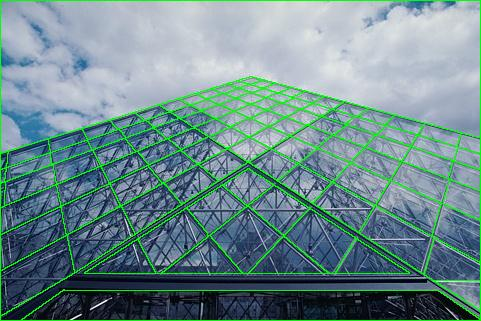
\includegraphics[scale=\scalefivebsd]{pictures/bsd-3-ground-truth-1}
	}
	\subfigure{
		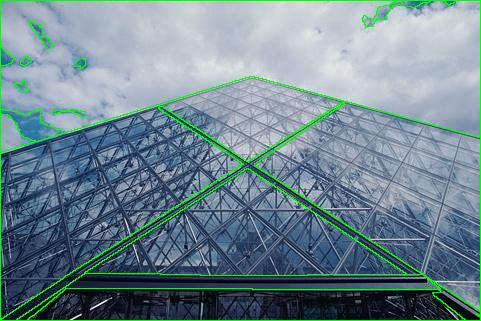
\includegraphics[scale=\scalefivebsd]{pictures/bsd-3-ground-truth-2}
	}
	\subfigure{
		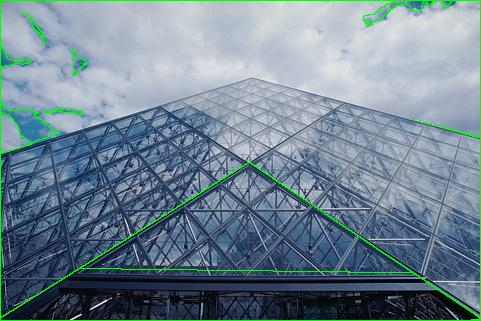
\includegraphics[scale=\scalefivebsd]{pictures/bsd-3-ground-truth-3}
	}
	\subfigure{
		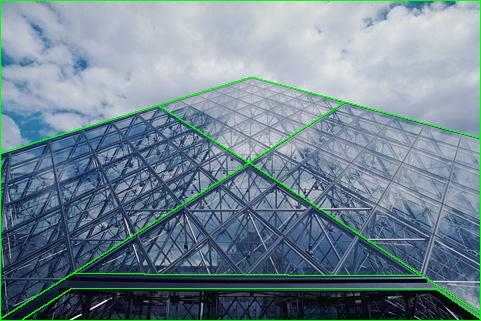
\includegraphics[scale=\scalefivebsd]{pictures/bsd-3-ground-truth-4}
	}
	\subfigure{
		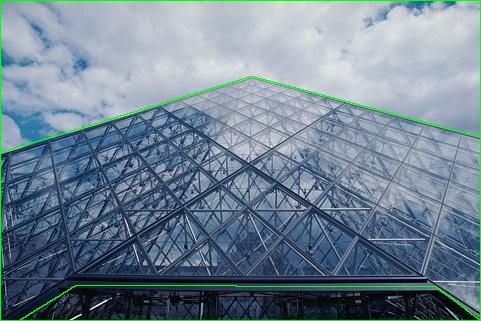
\includegraphics[scale=\scalefivebsd]{pictures/bsd-3-ground-truth-5}
	}
	\subfigure{
		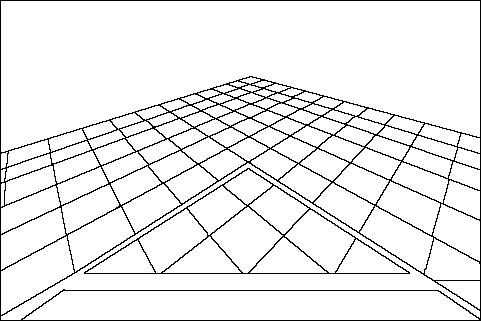
\includegraphics[scale=0.1535]{pictures/bsd-3-ground-truth-1-lines}
	}
	\subfigure{
		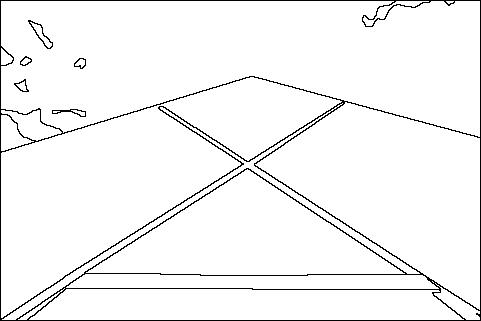
\includegraphics[scale=0.1535]{pictures/bsd-3-ground-truth-2-lines}
	}
	\subfigure{
		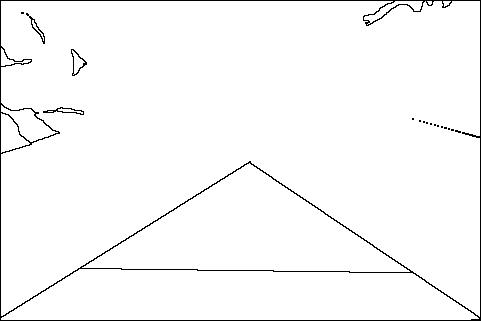
\includegraphics[scale=0.1535]{pictures/bsd-3-ground-truth-3-lines}
	}
	\subfigure{
		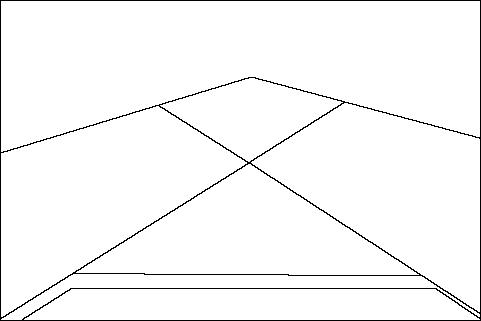
\includegraphics[scale=0.1535]{pictures/bsd-3-ground-truth-4-lines}
	}
	\subfigure{
		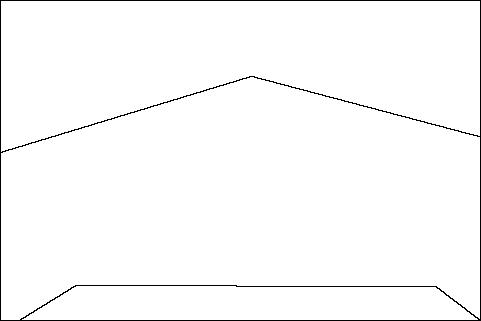
\includegraphics[scale=0.1535]{pictures/bsd-3-ground-truth-5-lines}
	}
	\caption[Several ground truth segmentations of one of the running examples as provided by the Berkeley Segmentation Dataset \cite{ArbelaezMaireFowlkesMalik:2011}.]{Ground truth segmentations of one of the running examples as provided by the BSDS500.}
	\label{fig:datasets-bsd-ground-truth}
\end{figure}
The first version of the Berkeley Segmentation Dataset, introduced in \cite{MartinFowlkesTalMalik:2001} and referred to as BSDS300, comprises $300$ images split up into a training set of $200$ images and a test set of $100$ images. The second version \cite{ArbelaezMaireFowlkesMalik:2011}, referred to as BSDS500, adds $200$ additional images forming a new test set while the old test set is used as validation set instead. Per image, at least five ground truth segmentations are available, each annotated by a different person, see for example figure \ref{fig:datasets-bsd-ground-truth}. Therefore, the ground truth segmentations are highly varying and reflect the difficult nature of segmenting natural images. Overall, this results in a fair evaluation of superpixel algorithms as for each superpixel segmentation a suitable ground truth segmentation can be chosen or the average performance over the ground truth segmentations can be computed. In practice, concerning all measures based on ground truth segmentations presented in this chapter, for each image we choose the ground truth segmentation resulting in the best value and subsequently average over all images. However, note that some of the measures provided as part of the Berkeley Segmentation Benchmark offer natural extensions to multiple ground truth segmentations, as for example the Probabilistic Rand Index \cite{UnnikrishnanPantofaruHebert:2007}, see appendix \ref{chapter:appendix-berkeley-segmentation-benchmark}.
% The first version, referred to as BSDS300, comprises $300$ images and was introduced in \cite{MartinFowlkesTalMalik:2001}. The dataset is split into a training set of $200$ images and a test set of $100$ images. For each image there are five ground truth segmentations available. The second version, introduced in \cite{ArbelaezMaireFowlkesMalik:2011}, adds $200$ additional images and is referred to as BSDS500. The old test set forms a validation set and the new $200$ images form the new test set. We use the BSDS500 as it is provided (no pre-processing is necessary). The images have size $321 \times 481$ or $481 \times 321$ depending on the aspect ratio. Figures \ref{subfig:introduction-running-examples-bsd-1} - \ref{subfig:introduction-running-examples-bsd-3} are taken from the validation set of the BSDS500.
%Figure \ref{fig:datasets-berkeley-segmentation-dataset-ground-truth} shows two of the provided ground truth segmentation, respectively.
%\begin{figure}
%	\subfigure[]{
%		\label{subfig:datasets-berkeley-segmentation-dataset-ground-truth-1-1}
%		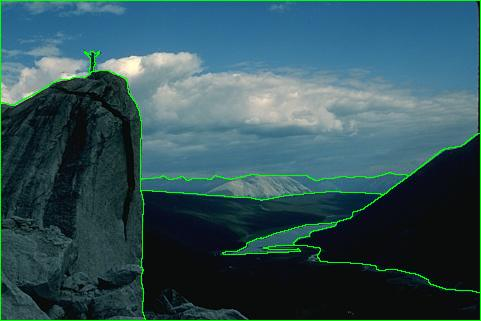
\includegraphics[scale=\scalethreebsd]{pictures/bsd-1-ground-truth-1}
%	}
%	\subfigure[]{
%		\label{subfig:datasets-berkeley-segmentation-dataset-ground-truth-2-1}
%		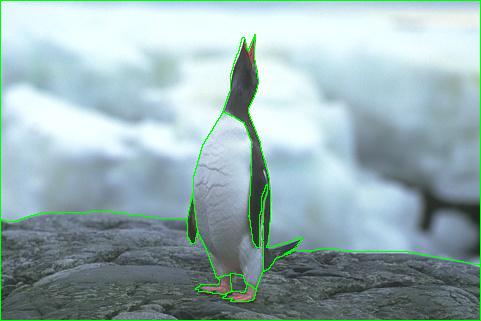
\includegraphics[scale=\scalethreebsd]{pictures/bsd-2-ground-truth-1}
%	}
%	\subfigure[]{
%		\label{subfig:datasets-berkeley-segmentation-dataset-ground-truth-3-1}
%		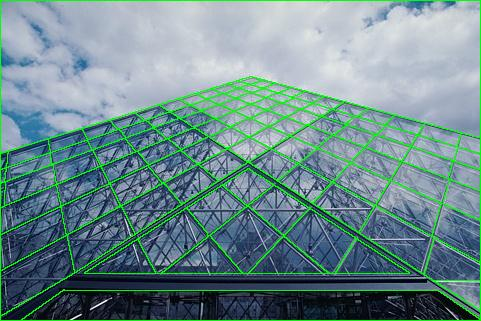
\includegraphics[scale=\scalethreebsd]{pictures/bsd-3-ground-truth-1}
%	}
%	\subfigure[]{
%		\label{subfig:datasets-berkeley-segmentation-dataset-ground-truth-1-2}
%		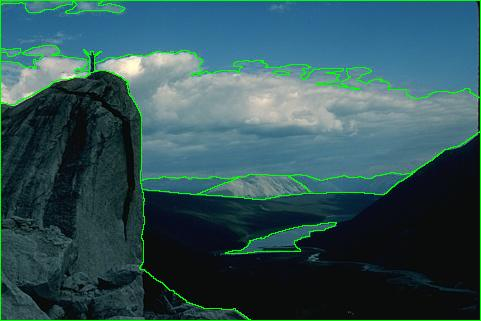
\includegraphics[scale=\scalethreebsd]{pictures/bsd-1-ground-truth-2}
%	}
%	\subfigure[]{
%		\label{subfig:datasets-berkeley-segmentation-dataset-ground-truth-2-2}
%		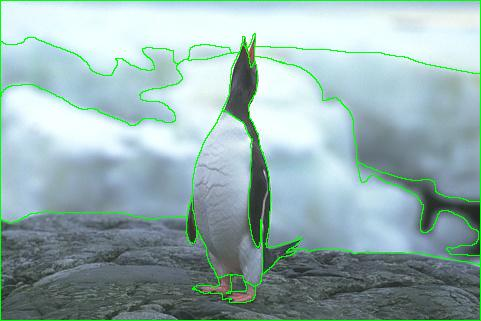
\includegraphics[scale=\scalethreebsd]{pictures/bsd-2-ground-truth-2}
%	}
%	\subfigure[]{
%		\label{subfig:datasets-berkeley-segmentation-dataset-ground-truth-3-2}
%		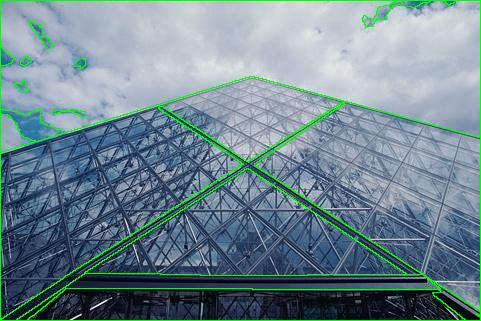
\includegraphics[scale=\scalethreebsd]{pictures/bsd-3-ground-truth-2}
%	}
%	\caption[Ground truth segmentations for the running examples as provided by the Berkeley Segmentation Dataset \cite{ArbelaezMaireFowlkesMalik:2011}.]{A selection of two ground truth segmentations of the running examples shown in figures \ref{subfig:introduction-running-examples-bsd-1} - \ref{subfig:introduction-running-examples-bsd-3}, respectively.}
%	\label{fig:datasets-berkeley-segmentation-dataset-ground-truth}
%\end{figure}

\begin{figure}[t]
	\centering
	\subfigure{
		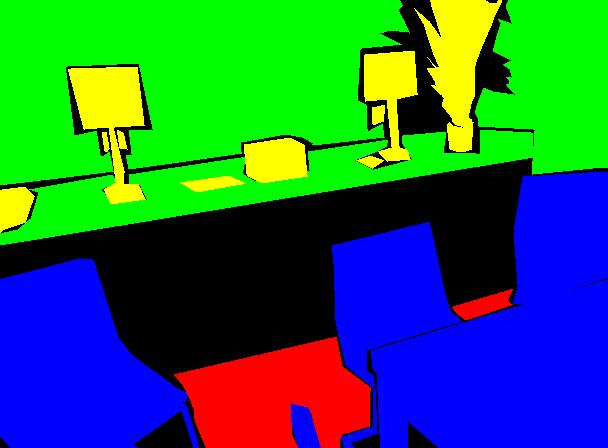
\includegraphics[scale=\scalefivenyu]{pictures/nyu-1-labels}
	}
	\subfigure{
		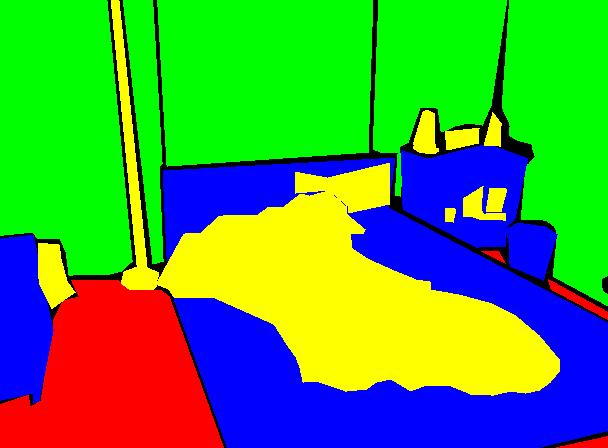
\includegraphics[scale=\scalefivenyu]{pictures/nyu-2-labels}
	}
	\subfigure{
		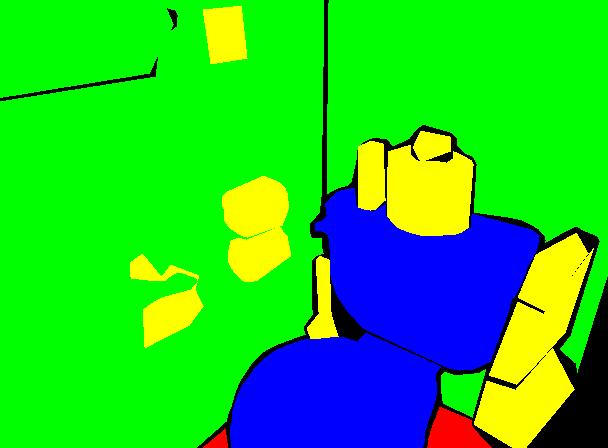
\includegraphics[scale=\scalefivenyu]{pictures/nyu-3-labels}
	}
	\subfigure{
		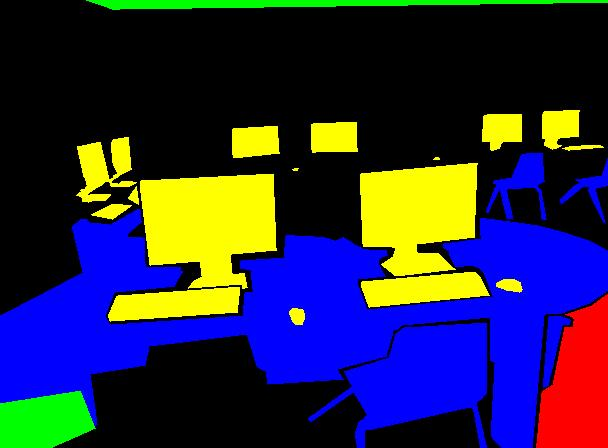
\includegraphics[scale=\scalefivenyu]{pictures/nyu-4-labels}
	}
	\subfigure{
		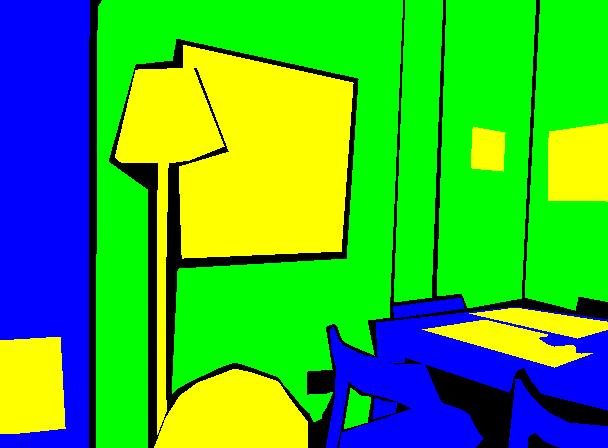
\includegraphics[scale=\scalefivenyu]{pictures/nyu-5-labels}
	}
	\subfigure{
		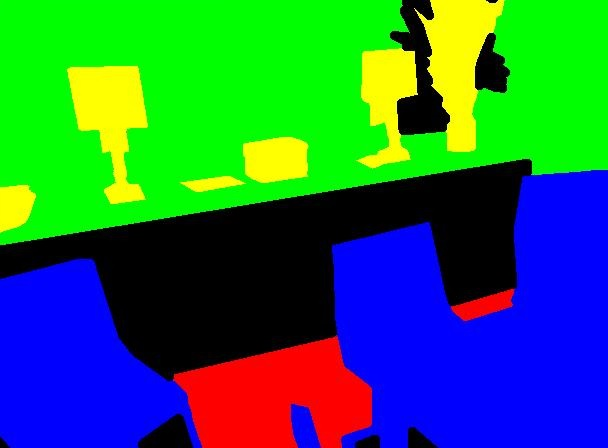
\includegraphics[scale=0.16]{pictures/nyu-1-labels-thinned}
	}
	\subfigure{
		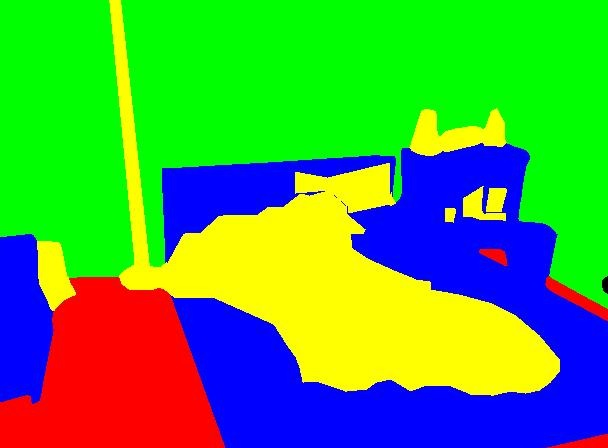
\includegraphics[scale=0.16]{pictures/nyu-2-labels-thinned}
	}
	\subfigure{
		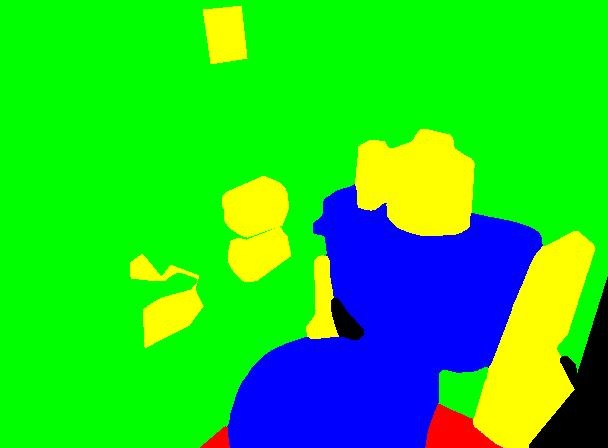
\includegraphics[scale=0.16]{pictures/nyu-3-labels-thinned}
	}
	\subfigure{
		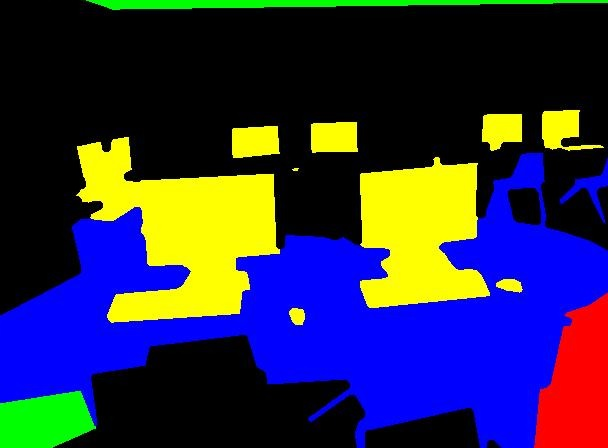
\includegraphics[scale=0.16]{pictures/nyu-4-labels-thinned}
	}
	\subfigure{
		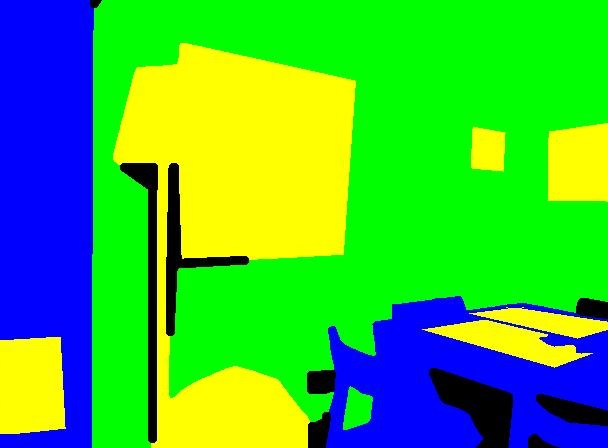
\includegraphics[scale=0.16]{pictures/nyu-5-labels-thinned}
	}
	\caption[Structure labels of the running examples as provided by the NYU Depth Dataset \cite{SilbermanHoiemKohliFergus:2012} and after removing small unlabeled regions in between larger labeled regions.]{The NYUV2 provides a high variety of different labels. In \cite{SilbermanHoiemKohliFergus:2012}, Silberman \etal grouped these labels to obtain a total of four so called structure labels. Top: the structure labels as provided by the NYUV2. Bottom: the structure labels after removing thin unlabeled regions in between larger labeled regions. Black indicates unlabeled pixels. Overall, this illustrates why the dataset is considered harder in comparison to the natural images from the BSDS500.}
	\label{fig:datasets-nyu-depth-dataset-labels}
\end{figure}
\section{NYU Depth Dataset}

The first version of the NYU Depth Dataset, in the following referred to as NYUV1, was introduced in \cite{SilbermanFergus:2011} by Silberman \etal. The dataset comprises $2284$\footnote{Although, Silberman \etal mention $2347$ labeled frames \cite{SilbermanFergus:2011}, we found that, actually, the dataset comprises only $2284$ labeled frames.} labeled frames taken from video sequences showing six different indoor scenes. The video sequences were taken by a calibrated Microsoft Kinect \cite{SilbermanFergus:2011} such that depth information is accessible. The frames were annotated using the LabelMe tool \cite{RussellTorralbaMurphyFreeman:2008} resulting in around $1000$ classes which are highly redundant \cite{SilbermanFergus:2011}.

The second version of the NYU Depth Dataset \cite{SilbermanHoiemKohliFergus:2012}, NYUV2, adds further variety in the form of indoor scenes from different cities as well as commercial accommodations. The dataset comprises $1449$ labeled frames with a total of $894$ classes \cite{SilbermanHoiemKohliFergus:2012}. Every instance of a particular class within a single frame gets a unique instance label. Following Ren and Bo \cite{RenBo:2012} we combine class labels and instance labels to generate ground truth segmentations compatible with the Berkeley Segmentation Benchmark. Although Silberman \etal state that the annotators were instructed to provide a dense labeling of the scenes, the images often contain small unlabeled regions in between larger labeled regions, see figure~\ref{fig:datasets-nyu-depth-dataset-labels}. Therefore, based on code provided by Ren and Bo \cite{RenBo:2012}, we remove these small background regions. Furthermore, bad lighting as well as cluttered scenes account for the difficulty of the NYUV2. However, this also represents an appropriate contrast to the natural images of the BSDS500.
% Therefore, based on the measures introduced in section \ref{section:datasets-extended-berkeley-segmentation-benchmark}, the dataset is overall harder to oversegment. However, this may also be due to the chosen scenes. In contrast to the BSDS500, the NYU Depth Dataset contains indoor scenes which are mostly untidy and highly cluttered. Additionally, only one ground truth segmentation per frame is provided. 

\begin{figure}[t]
	\centering
	\subfigure{
		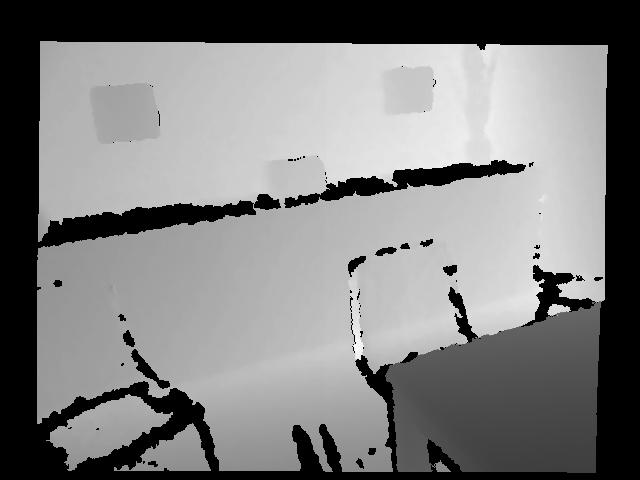
\includegraphics[scale=\scalefiveoriginalnyu]{pictures/nyu-1-raw-depth}
	}
	\subfigure{
		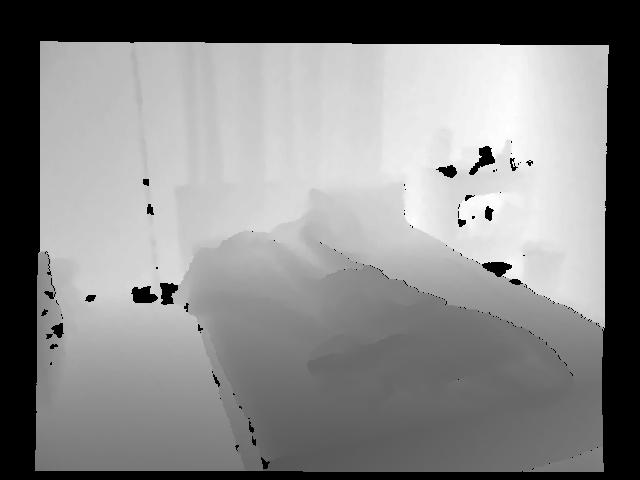
\includegraphics[scale=\scalefiveoriginalnyu]{pictures/nyu-2-raw-depth}
	}
	\subfigure{
		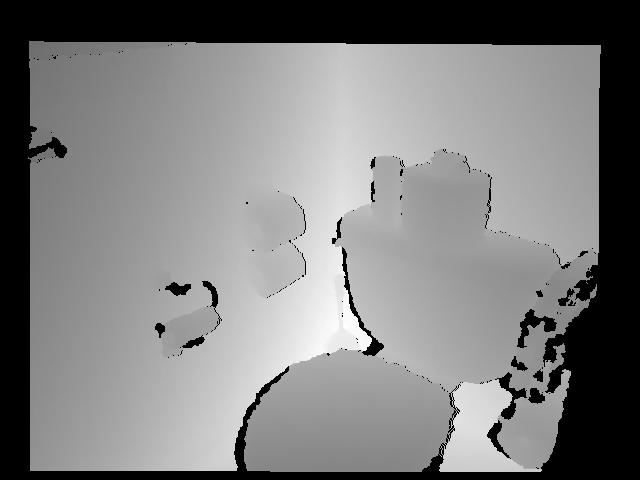
\includegraphics[scale=\scalefiveoriginalnyu]{pictures/nyu-3-raw-depth}
	}
	\subfigure{
		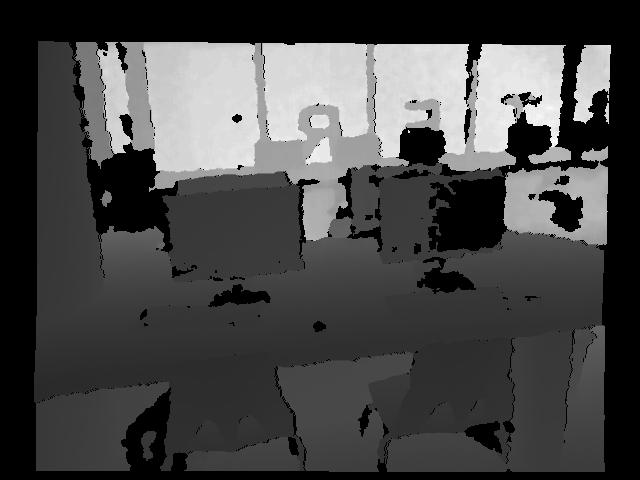
\includegraphics[scale=\scalefiveoriginalnyu]{pictures/nyu-4-raw-depth}
	}
	\subfigure{
		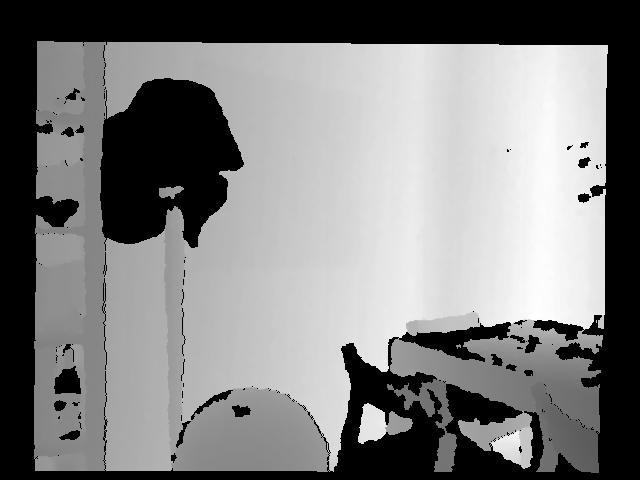
\includegraphics[scale=\scalefiveoriginalnyu]{pictures/nyu-5-raw-depth}
	}
	\subfigure{
		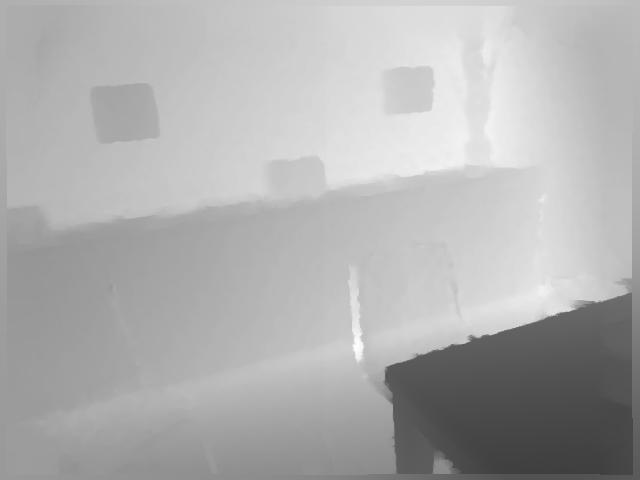
\includegraphics[scale=\scalefiveoriginalnyu]{pictures/nyu-1-depth}
	}
	\subfigure{
		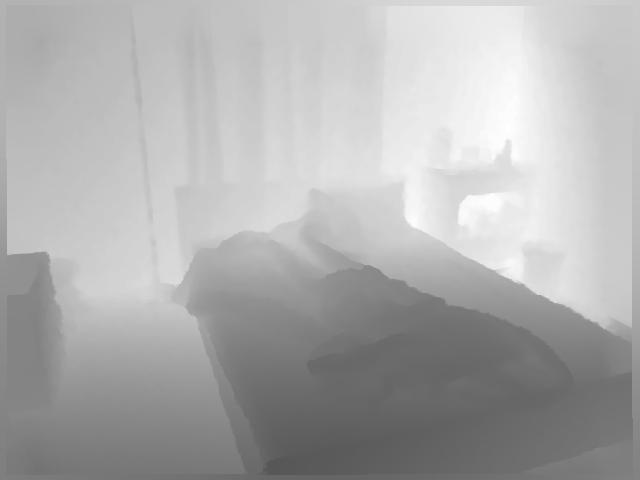
\includegraphics[scale=\scalefiveoriginalnyu]{pictures/nyu-2-depth}
	}
	\subfigure{
		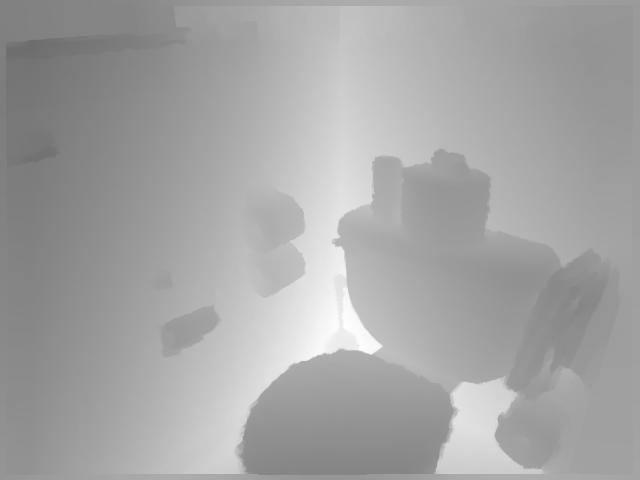
\includegraphics[scale=\scalefiveoriginalnyu]{pictures/nyu-3-depth}
	}
	\subfigure{
		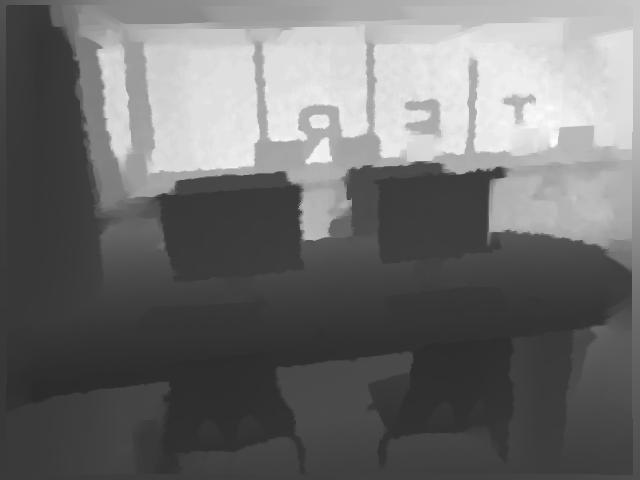
\includegraphics[scale=\scalefiveoriginalnyu]{pictures/nyu-4-depth}
	}
	\subfigure{
		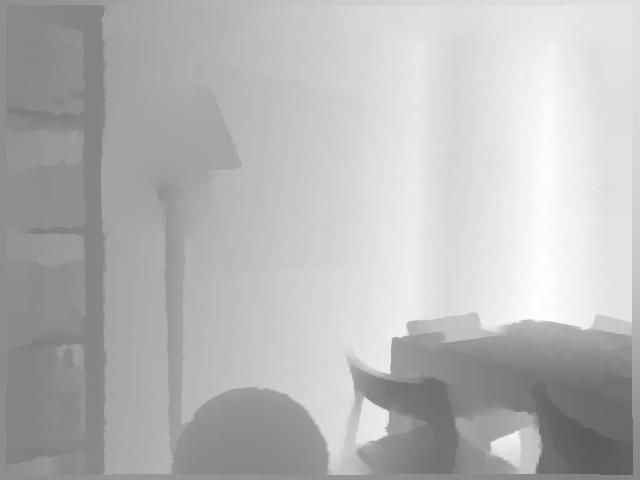
\includegraphics[scale=\scalefiveoriginalnyu]{pictures/nyu-5-depth}
	}
	\caption[The raw depth mages as well as the pre-processed depth images from the running examples as provided by the NYU Depth Dataset \cite{SilbermanHoiemKohliFergus:2012}.]{Top: the raw depth images corresponding to the running examples where black regions indicate that no depth information is available. Bottom: the pre-processed depth images corresponding to the running examples.}
	\label{fig:datasets-nyu-depth-dataset-depth}
\end{figure}

The NYUV2 includes both the raw depth images as well as a pre-processed version. The provided raw depth images have been aligned with the corresponding color images, however, the region covered by the depth images is significantly smaller and reflective surfaces such as mirrors and windows cause holes within the depth images. Therefore, Silberman \etal provide a pre-processed version of the depth images where these regions have been filled artificially. This is illustrated in figure \ref{fig:datasets-nyu-depth-dataset-depth}, showing both the raw depth images as well as the pre-processed depth images of the running examples. Furthermore, the provided images have been undistorted resulting in a small white border around the actual images. Therefore, we crop the images of size $640 \times 480$ to obtain images of size $608 \times 448$ without white borders. Finally, we choose $200$ images to form a training set and $400$ images to form a test set both including most of the available indoor scenes\footnote{Our split is based on a training/test split provided by Ren and Bo \cite{RenBo:2012}. However, to speed up evaluation, we reduced the size of the sets to $200$ and $400$, respectively. The images have been chosen such that almost all scenes are represented.}.

\section{Extended Berkeley Segmentation Benchmark}
\label{section:datasets-extended-berkeley-segmentation-benchmark}

Most measures provided as part of the Berkeley Segmentation Benchmark are unsuited for evaluating superpixel algorithms, see appendix \ref{chapter:appendix-berkeley-segmentation-benchmark}. Therefore, in this section, we discuss most of the available measures used to evaluate superpixel algorithms. These have, except for Boundary Recall, in the course of this thesis, been implemented into the framework of the Berkeley Segmentation Benchmark.

\subsection{Boundary Recall}

Boundary Recall is part of the Precision-Recall-Framework introduced in \cite{MartinFowlkesMalik:2004} which is discussed in detail in appendix \ref{chapter:appendix-berkeley-segmentation-benchmark}. Let $S$ be a superpixel segmentation and $G$ be a ground truth segmentation, then we define:
\begin{description}
 	\item[True Positives, $TP(S, G)$:] Boundary pixels in $G$ for which there is a boundary pixel in $S$ in range~$r$.
	\item[False Negatives, $FN(S, G)$:] Boundary pixels in $G$ for which there is no boundary pixel in $S$ in range~$r$.
\end{description}
where $r$ defines a tolerance parameter controlling the allowed deviation from the ground truth. In practice, $r$ is set to $0.0075$ times the image diagonal\footnote{This is the default value as used by the Berkeley Segmentation Benchmark and we chose not to change this value to keep our results comparable to other publications.}.
The Boundary Recall $Rec(S,G)$ is the fraction of all boundary pixels within the ground truth segmentation $G$ which are correctly detected within the superpixel segmentation $S$, that is
\begin{align}
	Rec(S,G) = \frac{|TP(S,G)|}{|TP(S,G)| + |FN(S,G)|}.
\end{align}
As we want superpixels to respect the boundaries within the image, a high Boundary Recall is desirable.

\subsection{Undersegmentation Error}
\label{subsection:datasets-extended-berkeley-segmentation-benchmark-undersegmentation-error}

The Undersegmentation Error describes the leakage or ``bleeding'' \cite{LevinshteinStereKutulakosFleetDickinsonSiddiqi:2009} of a superpixel with respect to a specific ground truth segment. In \cite{LiuTuzelRamalingamChellappa:2011} and \cite{VekslerBoykovMehrani:2010}, the Undersegmentation Error is defined as
\begin{align}
	\label{eq:datasets-extended-berkeley-segmentation-benchmark-ue-old}
	UE(S,G) = \frac{1}{N} \left( \sum_{G_i \in G} \left( \sum_{S_j \cap G_i \neq \emptyset} |S_j|\right) - N\right).
\end{align}
This equation computes the total amount of leakage for all ground truth segments and normalizes the sum by the number of pixels\footnote{We note that equation \eqref{eq:datasets-extended-berkeley-segmentation-benchmark-ue-old} uses a slightly different normalization when compared to the Undersegmentation Error as used by Levinshtein \etal in \cite{LevinshteinStereKutulakosFleetDickinsonSiddiqi:2009}.}. We note that the normalization used above may not be sufficient. For example consider a superpixel segmentation with a single superpixel covering the whole image. Then, if the ground truth consists of more than two segments, the Undersegmentation Error will be greater than one. In addition, as stated by Neubert and Protzel \cite{NeubertProtzel:2012} as well as Achanta \etal \cite{AchantaShajiSmithLucchiFuaSuesstrunk:2010} this definition has another serious disadvantage. Consider a large superpixel covering one ground truth segment perfectly except for some pixels. In the above equation, such superpixels receive high penalties \cite{NeubertProtzel:2012}. Achanta \etal adapt equation \eqref{eq:datasets-extended-berkeley-segmentation-benchmark-ue-old} to tolerate a small amount of leakage per superpixel:
\begin{align}
	UE(S,G) = \frac{1}{N} \left( \sum_{G_i \in G} \left( \sum_{|S_j \cap G_i| > B} |S_j|\right) - N\right)
\end{align}
where $B$ is the corresponding tolerance parameter. To avoid an additional parameter, we implemented the Undersegmentation Error as proposed by Neubert and Protzel:
\begin{align}
	\label{eq:datasets-extended-berkeley-segmentation-benchmark-ue}
	UE(S,G) = \frac{1}{N} \sum_{G_i \in G} \sum_{S_j \cap G_i \neq \emptyset} \min \{|S_j \cap G_i|, |S_j - G_i)\}.
\end{align}
where for each superpixel only the smaller part is considered leakage.

\subsection{Achievable Segmentation Accuracy}

When using superpixels as pre-processing step, we want the performance of subsequent steps to be as far as possible unaffected \cite{LiuTuzelRamalingamChellappa:2011}. Of course, as we inevitably loose information, this is not possible. However, we would like to quantify the accuracy achievable by subsequent steps, as for example classical segmentation. Achievable Segmentation Accuracy labels superpixels according to their underlying ground truth segments and counts the correctly labeled pixels \cite{LiuTuzelRamalingamChellappa:2011}:
\begin{align}
	ASA(S, G) = \frac{1}{N} \sum_{S_j \in S} \max_{G_i} \{|S_j \cap G_i|\}.
\end{align}
Therefore, Achievable Segmentation Accuracy represents an upper bound on the accuracy achievable by a subsequent segmentation step \cite{LiuTuzelRamalingamChellappa:2011}.

\subsection{Compactness}
\label{subsection:datasets-extended-berkeley-segmentation-benchmark-compactness}

Schick \etal \cite{SchickFischerStiefelhagen:2012} propose a compactness measure for superpixels based on the isoperimetric quotient. Given a superpixel $S_j$, the perimetric quotient relates the area $A(S_j)$ of the superpixel to the area of a circle with the same perimeter $U(S_j)$:
\begin{align}
	\frac{4\pi A(S_j)}{U(S_j)^2}.
\end{align}
As the circle represents the most compact form, the perimetric quotient measures the compactness of the superpixel, reaching $1$ if and only if the superpixel has the shape of a circle. The proposed compactness measure considers the perimetric quotient of all superpixels weighted by their area:
\begin{align}
	CO(S) = \frac{1}{N} \sum_{S_j \in S} |S_j| \frac{4 \pi A(S_j)}{U(S_j)^2}.
\end{align}
Although we assume superpixels to represent connected components, in practice, this will not always be the case. Therefore, we need to enforce connectivity before being able to compute the perimeter of the superpixels. Then, the above compactness measure captures the notion of spatial coherence within superpixels. The need of being able to measure compactness is also supported by Ren and Malik who introduce the concept of superpixels as ``local'' and ``coherent'' \cite{RenMalik:2003}.
% One problem with this measure is that calculating the perimeter for non-connected superpixels is not possible. Of course, this should not happen and in practice a superpixel with multiple components can be split up, however, this requires additional computation and post-processing. Also note that this measure is independent of a ground truth.% To date, this measure has only been used in \cite{HuazhuFuXiaochunCaoDaiTangYahongHanDongXu:2014}.

\subsection{Sum-of-Squared Error}

To measure the quality of the superpixel segmentation without being dependent on a ground truth, we propose to use the Sum-of-Squared Error as used for clustering evaluation as well:
\begin{align}
	SSE(S) = \frac{1}{N} \sum_{S_j \in S} \sum_{x_n \in S_j} d(x_n, S_j)^2
\end{align}
where $d(x_n, S_j)$ can be an arbitrary distance. In our case the euclidean distance in color space is suitable:
\begin{align}
	d(x_n, S_j) = \|I(x_n) - I(S_j)\|_2.
\end{align}
By coloring each pixel according to the corresponding superpixel's mean color, the superpixel segmentation is interpreted as reconstruction of the original image and the Sum-of-Squared Error measures the reconstruction error.

%The sum-of-squared error can also be used to evaluate the compactness of a superpixel segmentation when using
%\begin{align}
%	d(x_n, S_j) = \|x_n - \mu(S_j)\|_2.
%\end{align}
%However, $SSE(S)$ is comparably hard to interpret when using the above distance. To make the measure meaningful, we can normalize this by the number of pixels per superpixel and finally average over all superpixels:
%\begin{align}
%	SSE(S) = \frac{1}{K} \sum_{S_j \in S} \frac{1}{|S_j|} \sum_{x_n \in S_j} d(x_n, S_j)^2.
%\end{align}

\subsection{Explained Variation}

Another measure not depending on a ground truth segmentation is the Explained Variation. The Explained Variation quantifies how well the color variation within the image is captured by the superpixel segmentation \cite{HuazhuFuXiaochunCaoDaiTangYahongHanDongXu:2014}:
\begin{align}
	EV(S) = \frac{\sum_{S_j \in S} (I(S_j) - \mu)^2}{\sum_{n = 1}^N (I(x_n) - \mu)^2}
\end{align}
where $\mu$ is the mean color of the image. The information carried by an image is primarily defined by variation in color or intensity. Thus, Explained Variation measures the fraction of information captured by the superpixel segmentation.

%\section{Further Measures}
%
%There is an additional measure which is used only sporadically, for example in \cite{MoorePrinceWarrellMohammedJones:2008,DaiTangHuazhaFuXiaochunCao:2012} and \cite{HuazhuFuXiaochunCaoDaiTangYahongHanDongXu:2014}, called Size Variation.
%
%\subsection{Size Variation}
%
%The Size Variation tries to measure the regularity of a superpixel segmentation \cite{HuazhuFuXiaochunCaoDaiTangYahongHanDongXu:2014} using the variance of superpixel sizes:
%\begin{align}
%	SV(S) = \sum_{S_j \in S} (|S_j| - \frac{1}{K} \sum_{S_j \in S} |S_j|)^2.
%\end{align}
%However, we need to remember that this measure does not quantify the compactness or quality in any way. That is, the reason for varying superpixel sizes is not considered as part of this measure.